\documentclass[12pt]{article}
\usepackage{amsmath, amssymb, graphicx, geometry, setspace}
\usepackage{titlesec}
\usepackage{caption}
\usepackage{hyperref}
\usepackage{natbib}
\usepackage{placeins}  % �� NEW: controls float placement
\geometry{margin=1in}
\setstretch{1.25}

\titleformat{\section}{\large\bfseries}{\thesection.}{0.5em}{}
\titleformat{\subsection}{\normalsize\bfseries}{\thesubsection.}{0.5em}{}

\title{\textbf{Statistical Modeling of Volatility and Regime Switching in Financial Markets}\\
\large Volatility Clustering and Hidden Regime Dynamics in SPX and BTC}
\author{Ekantheswar Bandarupalli}
\date{October 2025}

\begin{document}
\maketitle

\begin{abstract}
We study volatility dynamics and regime behavior in equity and crypto markets by combining conditional volatility models from financial econometrics with hidden-state regime models from time-series inference. Using daily S\&P 500 proxy (SPY) and Bitcoin (BTC-USD) returns from 2015 to 2025, we estimate GARCH-family processes (GARCH(1,1), EGARCH, and GJR-GARCH) to model volatility clustering, and a Gaussian Hidden Markov Model (HMM) to infer latent market regimes (high-volatility vs. low-volatility states). Our results show that BTC’s volatility regimes are more persistent and asymmetric compared to SPY, providing evidence that crypto markets follow structurally different volatility dynamics.
\end{abstract}

\section{Introduction}
Financial markets exhibit volatility clustering—periods of calm followed by bursts of turbulence. Traditional constant-variance models fail to capture this dynamic. Bitcoin, in particular, demonstrates extreme tail behavior and regime persistence compared to equities.

This work aims to:
\begin{enumerate}
    \item Model how volatility evolves through time using econometric models (ARCH/GARCH family).
    \item Identify hidden market regimes through a Gaussian Hidden Markov Model (HMM).
\end{enumerate}

By contrasting SPY and BTC, we highlight how volatility persistence and transition probabilities differ between established and emerging asset classes.

\section{Related Work}
\citet{engle1982arch} introduced ARCH models where volatility depends on past shocks. \citet{bollerslev1986garch} extended this to GARCH to capture persistence. \citet{nelson1991egarch} and \citet{gjr1993} developed asymmetric GARCH variants (EGARCH, GJR-GARCH) to model leverage effects. 

\citet{hamilton1989ms} introduced regime-switching models, showing that macroeconomic and financial time series alternate between distinct latent states. Subsequent literature combines volatility modeling with regime inference to analyze crises, volatility bursts, and contagion.

\FloatBarrier
\section{Data}
We use daily adjusted close prices for:
\begin{itemize}
    \item SPY (S\&P 500 ETF as an equity proxy)
    \item BTC-USD (Bitcoin as a crypto proxy)
\end{itemize}

Data are retrieved from Yahoo Finance using \texttt{yfinance} from January 1, 2015, through October 2025. Log returns are computed as:
\begin{equation}
r_t = \log(P_t) - \log(P_{t-1})
\end{equation}

All datasets are aligned by timestamp and saved as \texttt{spx.csv}, \texttt{btc.csv}, and \texttt{aligned\_returns.csv}.

\FloatBarrier
\section{Methodology}
\subsection{GARCH-family Models}
We estimate three conditional volatility specifications for each asset:
\begin{itemize}
    \item \textbf{GARCH(1,1)}: Baseline model capturing volatility persistence.
    \item \textbf{EGARCH(1,1)}: Captures asymmetric (leverage) effects.
    \item \textbf{GJR-GARCH(1,1)}: Alternative asymmetric specification.
\end{itemize}

Conditional variance equation:
\begin{equation}
\sigma_t^2 = \omega + \alpha \varepsilon_{t-1}^2 + \beta \sigma_{t-1}^2
\end{equation}

Volatility forecasts are compared to realized 5-day volatility:
\begin{equation}
RV_t = \sqrt{\sum_{i=t-4}^{t} r_i^2}
\end{equation}

\FloatBarrier
\subsection{Hidden Markov Model (Regime Switching)}
We fit a 2-state Gaussian HMM to returns and squared returns:
\begin{itemize}
    \item State 0: low-volatility regime
    \item State 1: high-volatility regime
\end{itemize}

Transition matrix:
\begin{equation}
T_{ij} = P(s_{t+1}=j | s_t=i)
\end{equation}

\FloatBarrier
\section{Empirical Results}
\subsection{Volatility Clustering}
All GARCH-family models detect strong volatility clustering in both SPY and BTC. BTC’s conditional volatility is higher and more erratic, reflecting less mean reversion.

\begin{figure}[h!]
\centering
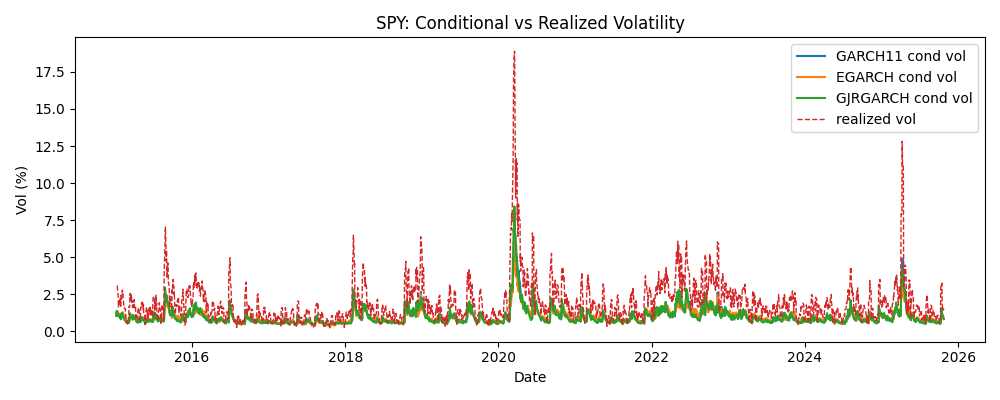
\includegraphics[width=0.8\textwidth]{SPY_cond_vs_realized.png}
\caption{SPY Conditional vs Realized Volatility}
\end{figure}

\begin{figure}[h!]
\centering
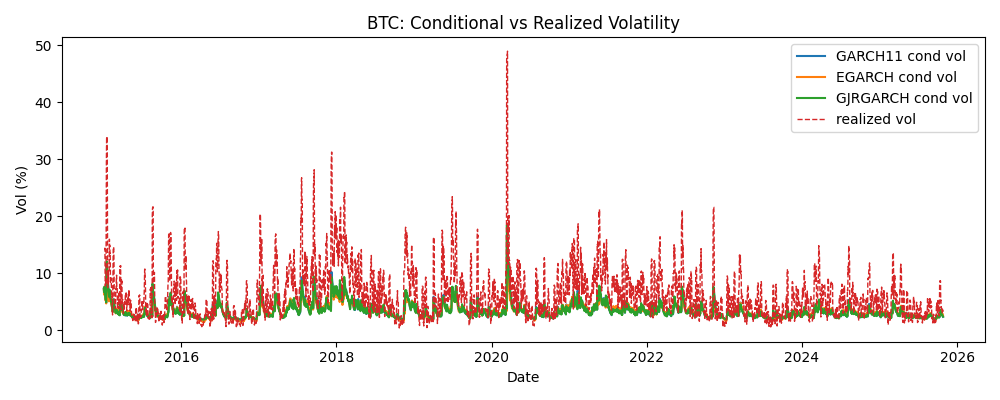
\includegraphics[width=0.8\textwidth]{BTC_cond_vs_realized.png}
\caption{BTC Conditional vs Realized Volatility}
\end{figure}

\FloatBarrier
\subsection{Regime Structure}
The HMM identifies two regimes in both assets: SPY exhibits short, frequent transitions, whereas BTC remains longer in high-volatility states.

\begin{figure}[h!]
\centering
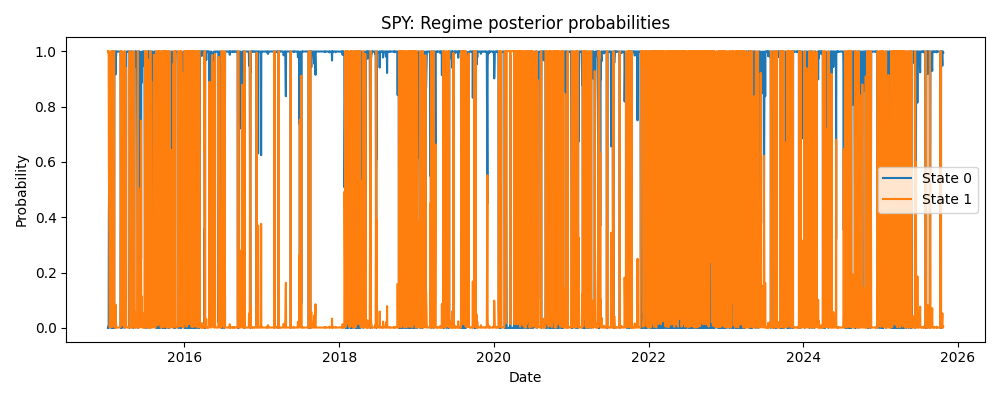
\includegraphics[width=0.8\textwidth]{SPY_regime_probs.png}
\caption{SPY Regime Posterior Probabilities}
\end{figure}

\begin{figure}[h!]
\centering
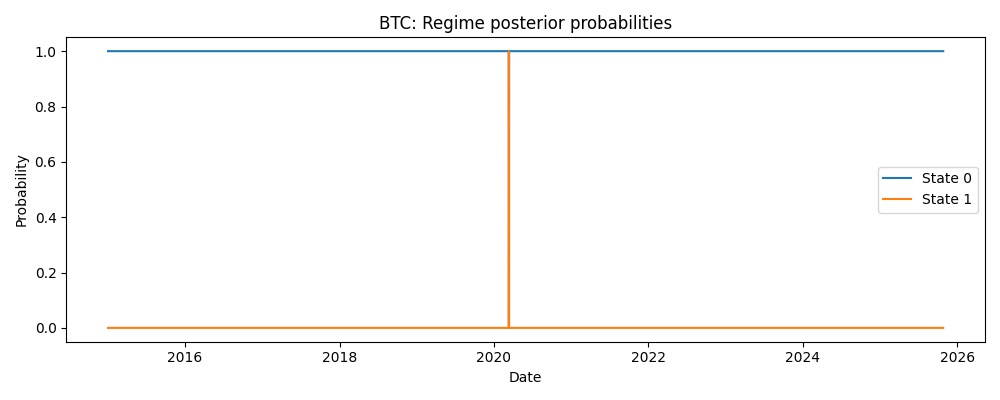
\includegraphics[width=0.8\textwidth]{BTC_regime_probs.png}
\caption{BTC Regime Posterior Probabilities}
\end{figure}

BTC’s high-volatility regime is ``stickier,'' suggesting prolonged stress phases.

\FloatBarrier
\subsection{Forecast Evaluation}
Forecast accuracy is evaluated via RMSE between one-day-ahead volatility forecasts and realized volatility.

\FloatBarrier
\section{Discussion}
\begin{enumerate}
    \item BTC volatility is structurally distinct—more asymmetric and persistent.
    \item GJR-GARCH and EGARCH outperform symmetric GARCH models.
    \item Regime models improve interpretability by identifying market states.
\end{enumerate}

This framework extends naturally to risk management, portfolio hedging, and reinforcement-learning trading systems.

\FloatBarrier
\section{Conclusion}
We presented a comparative study of volatility dynamics across SPY and BTC using GARCH-family and HMM models. Volatility clustering and asymmetry are more pronounced in BTC, while regime-switching models reveal persistent high-volatility states. 

Future research can integrate these latent regimes into algorithmic trading strategies using regime probabilities as risk-sensitive signals.

\FloatBarrier
\bibliographystyle{apalike}
\bibliography{refs}

\end{document}
